\chapter{Conclusion}
\section{Introduction}
This chapter contains reflections on the work that has been done, what can be done in the future that can strengthen the thesis

\section{Reflection}


\section{The Work Process}
\subsection{Meetings}
The team held meetings with their supervisor, Filip Holik, on a weekly basis. Although the meetings were typically scheduled for Wednesdays, they had to be postponed or canceled on occasion due to various circumstances. Meeting Minutes with the supervisor can be found in Appendix \ref{supervisormeeting}.
\\~\\
During the early stages of the project, the team met with the stakeholder every other week. However, as the project progressed, both parties agreed that weekly meetings would be beneficial. As the demand for help grew, the group required more regular assistance. Meeting Minutes with the stakeholder can be found in Appendix \ref{nbimmeeting}.  

\subsection{Scrum}


\subsection{Coordinated schedule}
Because the team members were involved in other activities such as jobs and involvement in the student association, it was important for them to coordinate their schedules. This method allowed the team to organize meetings more effectively and determine each member's availability for work. The team scheduled all of their activities and workdays using the calendar feature of their Teams channel.

\subsection{Draft Submissions}
The team set specified deadlines for producing multiple drafts at the start of the project. This approach tried to maintain constant development while avoiding last-minute delays. For instance, the group set an April 1st target for their first draft, which they were able to meet. As a result, both the supervisor and the stakeholder received the first draft on time. After a few days, the team got feedback and proceeded with their work. 

The team established a deadline for the final draft, which was the second for the project. In order to give the supervisor and stakeholders enough time to thoroughly read the thesis before the submission date on the 22nd of May, the team established the deadline for the final draft on the 1st of May, three weeks before the submission date. 


\subsection{Gantt Chart}
Since the group decided to do some changes to the scope during the project period, the original Gantt chart could not be followed. 

The research on tools was considered to be time-consuming at first, but with the changes made, this activity ended up being a smaller part of the thesis than anticipated. As a result, it took less time than what was first estimated. Furthermore, the \say{Testing tools}activity was removed since the team wanted to focus less on testing tools and more on integrating testing of the various tools into the pipeline-building process. 

Setting up the configuration of the pipeline with Terraform ended up being a much longer process than planned. 

However, what the group managed to follow was the planned deadlines for the different draft submissions. The first draft was delivered on the 3rd of April in week 13, and the final draft on the 2nd of May.

\vspace{2mm}
\begin{figure}[H]
    \centering
    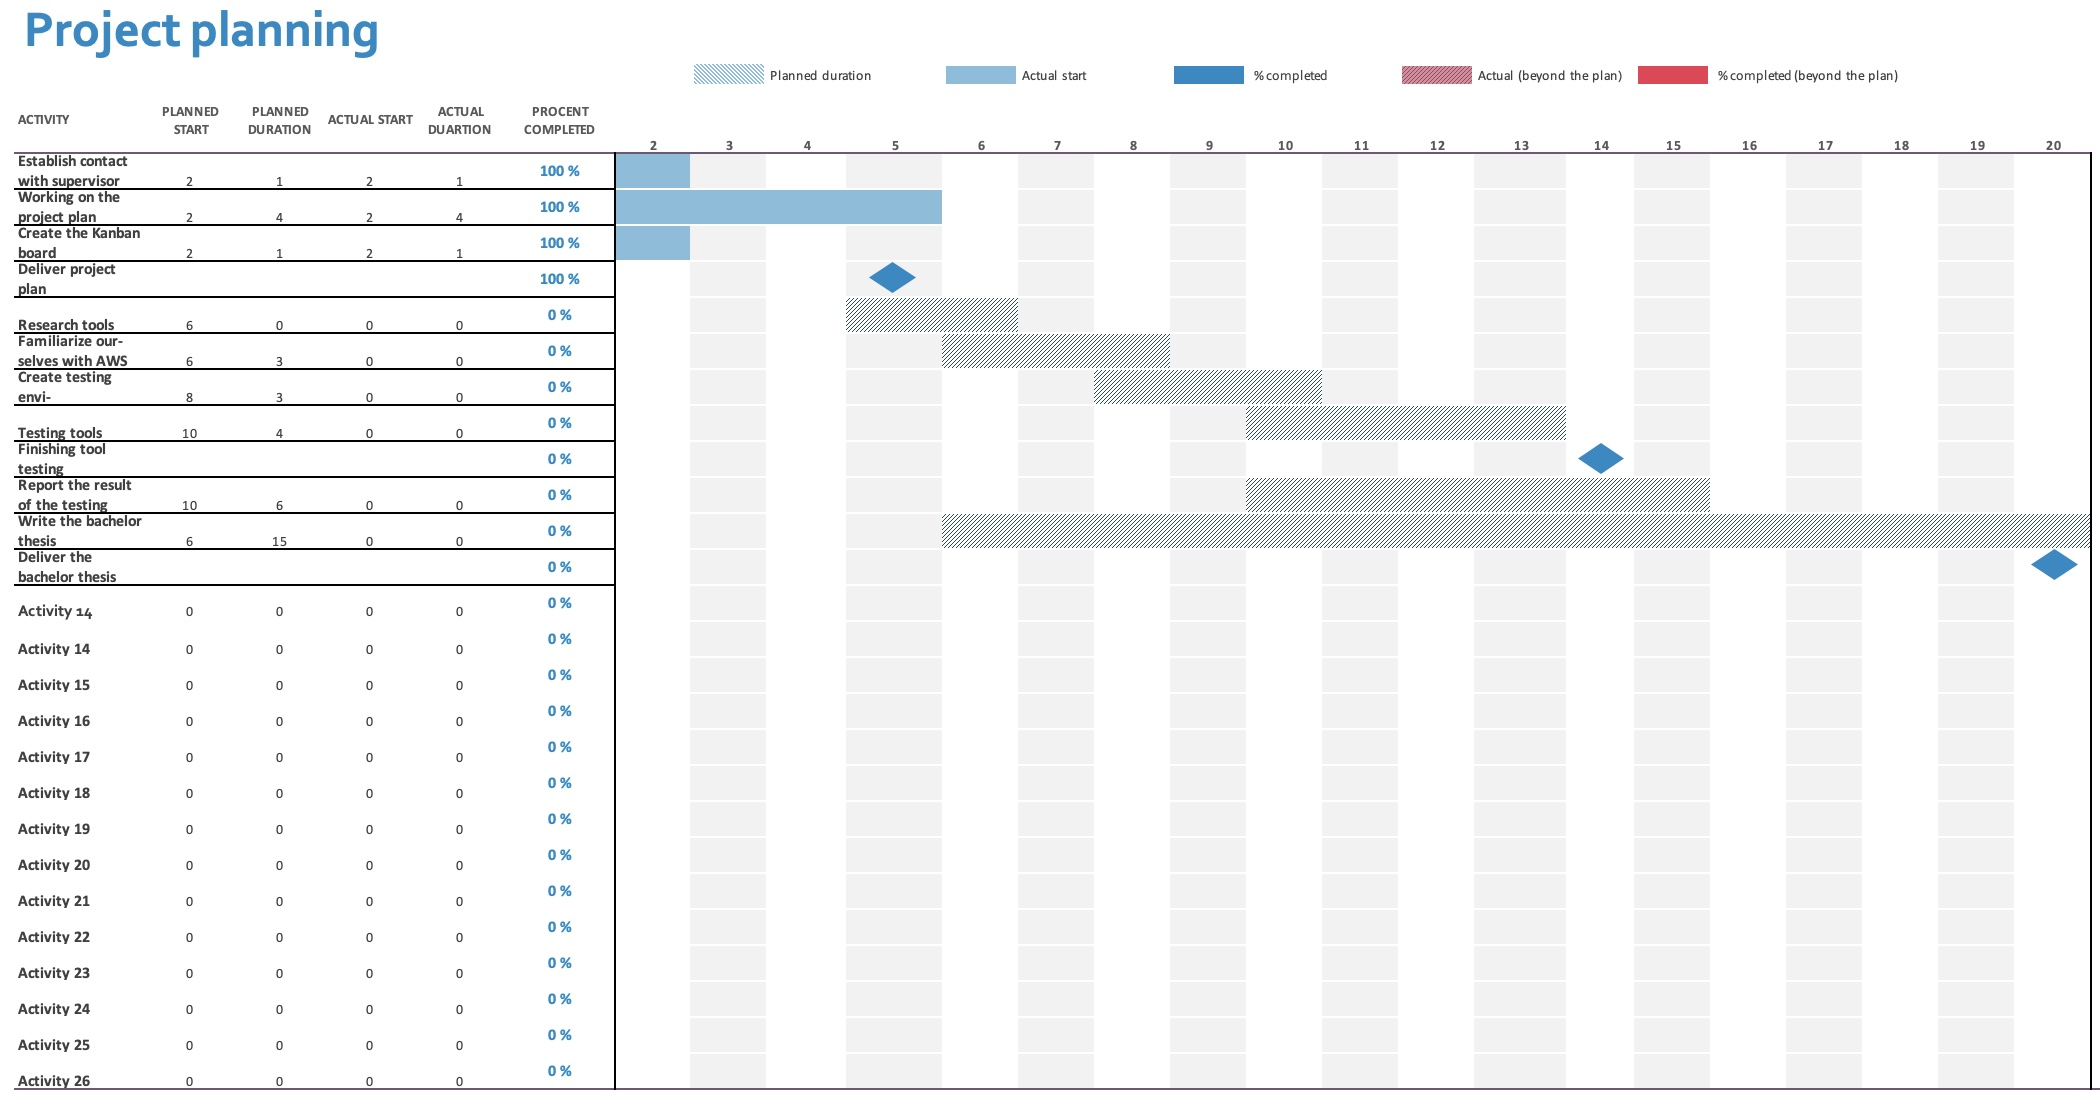
\includegraphics[width=0.8\columnwidth]{Images/gantt2.jpg}
    \caption{Original Gantt Chart}
    \label{fig: Original Gantt Chart}
\end{figure}

% Add a photo of the updated and finished Gantt chart

\subsection{Distribution of Work}
The group decided to divide the work into two parts at the start of the thesis to ensure that the thesis progressed continuously. The first part is practical, and the second is report writing. The responsibilities were assigned based on each group member's strength and what they most desired to do. Every member of the group contributed to the thesis, and everyone worked together to complete the report on time. 


\subsection{Goals}
%diskutere målene vi satt oss (vet ikke om det er nødvendig)



\section{Further Work}

In further work, it could strengthen the thesis to perform a broader analysis of various security tools that perform SAST, DAST, and SCA scans -  where the selected tools are based on these analyses. During these analyses, an assessment can also be made of which requirements must be met in order for a tool to be selected. 
\\~\\
To get an understanding of the whole \acrlong{sdlc}, it would have been relevant to add earlier phases into the thesis to acquire a more complete view of the life cycle and correspond with the shift-left method that prioritizes early testing to detect vulnerabilities sooner. This would demonstrate the shift-left concept, which involves conducting testing as early as feasible in the process.  

\section{Conclusion}
%snakke om hva vi har gjort og hva vi anbefaler 